% Figure from MATH 591 notes, section 61 (Lecture 21).
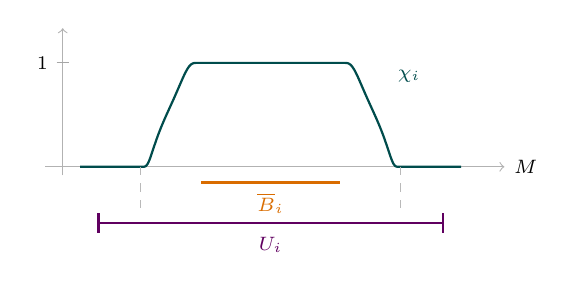
\begin{tikzpicture}[scale=1.1]
\draw[->, gray!60] (-2.6,0) -- (2.7,0) node[right, font=\scriptsize, text=black] {$M$};
\draw[->, gray!60] (-2.4,-0.1) -- (-2.4,1.6);
\draw[teal!60!black, thick] plot[smooth] coordinates {(-2.200,0.000) (-2.180,0.000) (-2.160,0.000) (-2.140,0.000) (-2.120,0.000) (-2.100,0.000) (-2.080,0.000) (-2.060,0.000) (-2.040,0.000) (-2.020,0.000) (-2.000,0.000) (-1.980,0.000) (-1.960,0.000) (-1.940,0.000) (-1.920,0.000) (-1.900,0.000) (-1.880,0.000) (-1.860,0.000) (-1.840,0.000) (-1.820,0.000) (-1.800,0.000) (-1.780,0.000) (-1.760,0.000) (-1.740,0.000) (-1.720,0.000) (-1.700,0.000) (-1.680,0.000) (-1.660,0.000) (-1.640,0.000) (-1.620,0.000) (-1.600,0.000) (-1.580,0.000) (-1.560,0.000) (-1.540,0.000) (-1.520,0.000) (-1.500,0.000) (-1.480,0.000) (-1.460,0.001) (-1.440,0.008) (-1.420,0.033) (-1.400,0.076) (-1.380,0.131) (-1.360,0.190) (-1.340,0.250) (-1.320,0.308) (-1.300,0.364) (-1.280,0.416) (-1.260,0.466) (-1.240,0.514) (-1.220,0.560) (-1.200,0.605) (-1.180,0.649) (-1.160,0.693) (-1.140,0.737) (-1.120,0.781) (-1.100,0.826) (-1.080,0.872) (-1.060,0.918) (-1.040,0.964) (-1.020,1.010) (-1.000,1.054) (-0.980,1.095) (-0.960,1.131) (-0.940,1.160) (-0.920,1.181) (-0.900,1.193) (-0.880,1.199) (-0.860,1.200) (-0.840,1.200) (-0.820,1.200) (-0.800,1.200) (-0.780,1.200) (-0.760,1.200) (-0.740,1.200) (-0.720,1.200) (-0.700,1.200) (-0.680,1.200) (-0.660,1.200) (-0.640,1.200) (-0.620,1.200) (-0.600,1.200) (-0.580,1.200) (-0.560,1.200) (-0.540,1.200) (-0.520,1.200) (-0.500,1.200) (-0.480,1.200) (-0.460,1.200) (-0.440,1.200) (-0.420,1.200) (-0.400,1.200) (-0.380,1.200) (-0.360,1.200) (-0.340,1.200) (-0.320,1.200) (-0.300,1.200) (-0.280,1.200) (-0.260,1.200) (-0.240,1.200) (-0.220,1.200) (-0.200,1.200) (-0.180,1.200) (-0.160,1.200) (-0.140,1.200) (-0.120,1.200) (-0.100,1.200) (-0.080,1.200) (-0.060,1.200) (-0.040,1.200) (-0.020,1.200) (0.000,1.200) (0.020,1.200) (0.040,1.200) (0.060,1.200) (0.080,1.200) (0.100,1.200) (0.120,1.200) (0.140,1.200) (0.160,1.200) (0.180,1.200) (0.200,1.200) (0.220,1.200) (0.240,1.200) (0.260,1.200) (0.280,1.200) (0.300,1.200) (0.320,1.200) (0.340,1.200) (0.360,1.200) (0.380,1.200) (0.400,1.200) (0.420,1.200) (0.440,1.200) (0.460,1.200) (0.480,1.200) (0.500,1.200) (0.520,1.200) (0.540,1.200) (0.560,1.200) (0.580,1.200) (0.600,1.200) (0.620,1.200) (0.640,1.200) (0.660,1.200) (0.680,1.200) (0.700,1.200) (0.720,1.200) (0.740,1.200) (0.760,1.200) (0.780,1.200) (0.800,1.200) (0.820,1.200) (0.840,1.200) (0.860,1.200) (0.880,1.199) (0.900,1.193) (0.920,1.181) (0.940,1.160) (0.960,1.131) (0.980,1.095) (1.000,1.054) (1.020,1.010) (1.040,0.964) (1.060,0.918) (1.080,0.872) (1.100,0.826) (1.120,0.781) (1.140,0.737) (1.160,0.693) (1.180,0.649) (1.200,0.605) (1.220,0.560) (1.240,0.514) (1.260,0.466) (1.280,0.416) (1.300,0.364) (1.320,0.308) (1.340,0.250) (1.360,0.190) (1.380,0.131) (1.400,0.076) (1.420,0.033) (1.440,0.008) (1.460,0.001) (1.480,0.000) (1.500,0.000) (1.520,0.000) (1.540,0.000) (1.560,0.000) (1.580,0.000) (1.600,0.000) (1.620,0.000) (1.640,0.000) (1.660,0.000) (1.680,0.000) (1.700,0.000) (1.720,0.000) (1.740,0.000) (1.760,0.000) (1.780,0.000) (1.800,0.000) (1.820,0.000) (1.840,0.000) (1.860,0.000) (1.880,0.000) (1.900,0.000) (1.920,0.000) (1.940,0.000) (1.960,0.000) (1.980,0.000) (2.000,0.000) (2.020,0.000) (2.040,0.000) (2.060,0.000) (2.080,0.000) (2.100,0.000) (2.120,0.000) (2.140,0.000) (2.160,0.000) (2.180,0.000) (2.200,0.000)};
\node[teal!60!black, font=\scriptsize] at (1.6,1.05) {$\chi_i$};
\draw[gray!70] (-2.47,1.2) -- (-2.33,1.2) node[left, xshift=-4pt, font=\scriptsize, text=black] {$1$};
\draw[orange!85!black, very thick] (-0.8,-0.18) -- (0.8,-0.18); \node[orange!85!black, font=\scriptsize] at (0,-0.42) {$\overline{B}_i$};
\draw[violet!75!black, thick, |-|] (-2.0,-0.65) -- (2.0,-0.65); \node[violet!75!black, font=\scriptsize] at (0,-0.9) {$U_i$};
\draw[gray!55, dashed] (-1.5,0) -- (-1.5,-0.55); \draw[gray!55, dashed] (1.5,0) -- (1.5,-0.55);

\end{tikzpicture}
